\setcounter{chapter}{-1}

\chapter{一些约定与预备知识}
\label{cha:first-things-first}

俗话说,「磨刀不误砍柴工」。在一切开始之前,我们先对本书中的一些标记和约定进行说明,同时为你提供一些可能有助于你更好地阅读本书的预备知识。

\section{《你缺计课》是什么}

《你缺计课》是一门\regcolor{面向当下的「零门槛」电脑课}:《你缺计课》旨在帮助你轻松掌握「如何在当下更高效地使用电脑」。如果你是电脑小白,本书会手把手地引导你迈入数字世界;如果你已经熟悉电脑操作,它也能助你发现可能忽略的小技巧,查漏补缺。

《你缺计课》是一本\regcolor{展望未来的「信息化」科普书}:从计算技术到人工智能,从云计算到网络安全,本书以通俗易懂的语言,带你探索这些塑造当今与未来的核心技术,让你对信息化世界有更清晰的认识。

\section{《你缺计课》不是什么}

《你缺计课》\regcolor{不是任何软件的使用手册}:本书不会详细讲解某款软件的具体操作方法。相反,我们更注重帮助你理解各种软件的功能、特点以及它们在不同场景中的作用。

《你缺计课》\regcolor{不是大部头而死板的教材}:有别于枯燥、繁琐而呆板的专业教材,本书希望和你成为朋友,与你一同踏上一场轻松愉快的旅程。它轻松、有趣、接地气,贴近生活,伴你前行。

\section{文中的标记符号}

在《你缺计课》中,我们使用方头括号「【】」来标记所有屏幕上字面显示的选项。例如,当我们希望你右键桌面上的图标
\begin{figure}[htb!]
  \centering
  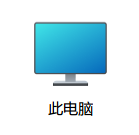
\includegraphics[width=2cm]{assets/basic/This_PC.png}
\end{figure}

\noindent 时,我们会称「右键【此电脑】」。

我们使用右箭头「→」来表示下一步操作。例如,「右键【此电脑】→【属性】」的意思是,右键桌面上的【此电脑】图标,然后在弹出的菜单中点击【属性】。

如果某一章节的标题后带有星号「*」,表明这一章节内容可能较难理解,可以选择性阅读。

本书中的链接会以这种样式呈现:\url{https://missing.criwits.top/}。

\begin{note}
  有这种特殊外框的文字,通常是一些题外话。它们可能是一些供你思考的问题,或是一些有助于理解正文的额外知识。
\end{note}

\section{快捷键的操作说明}

如果你按快捷键(组合键)后,电脑并没有行使预想的功能,可能是你的按法不对。快捷键的按法并不是「同时按下所有的键」,而是「依展示次序按下各键不松手,最后一起松开」。例如,若要按快捷键「\keys{\Windows + Shift + S}」:

\begin{itemize}
  \item 先按住 \keys{\Windows} 键(\keys{\Windows} 键上印有Window 徽标「\Windows」或「\WindowsTen」,一般来说这个键在 \keys{Ctrl} 和 \keys{Alt} 之间)不要松手;
  \item 再按住 \keys{Shift} 键,同样不要松手;
  \item 接着按一下 \keys{S} 键,然后松开全部按键。
\end{itemize}

\section{\keys{F1} -- \keys{F12} 功能键的使用说明}

在很久以前,人们为了增加电脑键盘的使用效率,在键盘的最顶端设计了一排按键,它们就是 \keys{F1} -- \keys{F12} 功能键。这些功能键和键盘上的 \keys{Ctrl}、\keys{Alt} 等键一样,并不能用来输入文字,而是用来组合出各种功能的。比如,\keys{Alt + F4} 可以用来关闭当前程序,\keys{F5} 可以用来刷新网页,\keys{F1} 用来查找帮助等。

随着电脑操作方式不断演进,\keys{F1} -- \keys{F12} 键使用得越来越少。这时,人们想,与其让这些键在键盘上吃灰,不如赋予它们一些新功能,比如快捷调整屏幕亮度、音量、无线网络连接等设置。于是,一些电脑键盘,尤其是笔记本电脑的键盘上,这 12 个按键在它们原本的功能之外,增加了一层「扩展功能」。

\begin{figure}[htb!]
  \centering
  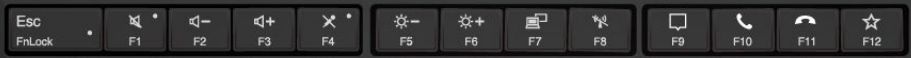
\includegraphics[width=.9\textwidth]{assets/basic/F1_to_F12_keys_with_extra_functions.png}
  \caption{带有额外功能的 F1—F12 功能键}
  \label{fig:F1_to_F12_keys_with_extra_functions}
\end{figure}

上图展示的就是 \keys{F1} -- \keys{F12} 键拥有扩展功能的键盘。这里,\keys{F1} -- \keys{F12} 这些键上被画上了一些符号。这些符号代表了这些键的扩展功能。例如,上图中 \keys{F5} 键上画有亮度降低的符号,因此 \keys{F5} 键的扩展功能就是降低屏幕亮度; \keys{F1} 键画有静音的符号,因此 \keys{F1} 键的扩展功能就是静音。

为了让 \keys{F1} -- \keys{F12} 键能够在这两种功能中自如切换,人们在键盘左下角安排了一个 \keys{Fn} 键(意思是 function,功能)。具体地,对于一台具有 \keys{Fn} 键的电脑,它的键盘情况是下列两种情况中的一种:

\begin{enumerate}
  \item 直接按 \keys{F1} -- \keys{F12} 功能键可以行使它们原本的功能,按住 \keys{Fn} 的同时再按 \keys{F1} -- \keys{F12} 则行使它们的扩展功能。例如:按 \keys{F5} 可以在浏览器中刷新页面(常见浏览器基本都可以),按 \keys{Fn + F5} 可以降低屏幕亮度。
  \item 直接按 \keys{F1} -- \keys{F12} 功能键可以行使它们的扩展功能,按住 \keys{Fn} 的同时再按 \keys{F1} -- \keys{F12} 则行使它们原本的功能。例如:按 \keys{F5} 可以降低屏幕亮度,按 \keys{Fn + F5} 可以在浏览器中刷新页面。
\end{enumerate}

\begin{figure}[htb!]
  \centering
  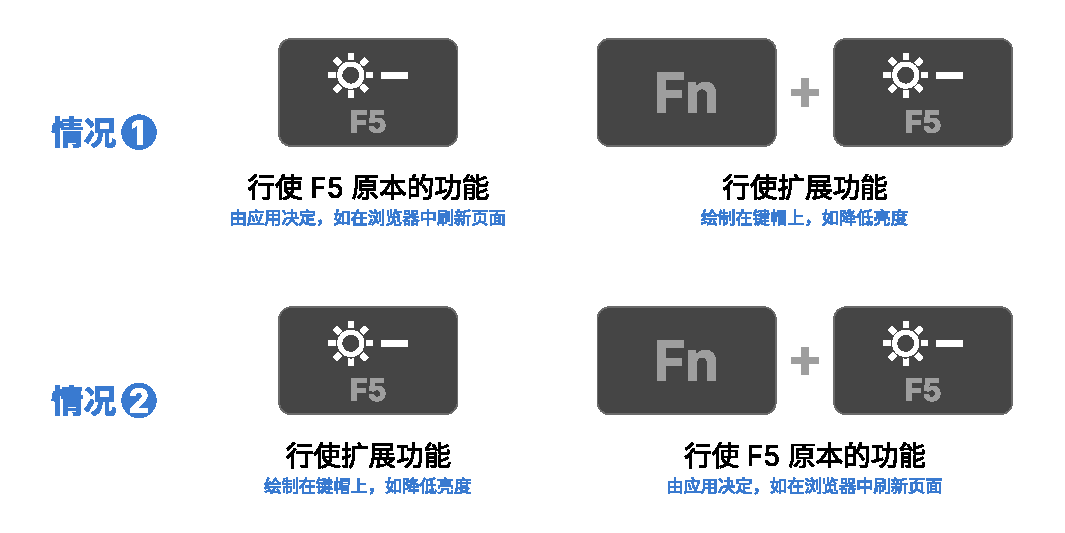
\includegraphics[width=.8\textwidth]{assets/basic/Fn_functions.pdf}
  \caption{\keys{F1} -- \keys{F12} 的两种功能情况}
  \label{fig:Fn_functions}
\end{figure}

你可以随便打开一个应用(比如浏览器),然后按 \keys{Alt + F4}。如果刚打开的应用退出了,就说明你的电脑属于上面两种情况中的第一种。如果没有反应,就属于第二种。

有些键盘提供了快捷的方法在这两种模式中切换。比如某些笔记本电脑键盘,可以通过按 \keys{Fn + Esc} 来切换这两种模式。另一些键盘可能需要使用专门的软件来进行调整,具体还请参考你的笔记本电脑或者键盘的说明书。

\begin{note}
	这意味着,对于那些包含 \keys{F1} -- \keys{F12} 功能键的快捷键,如果你按下后电脑没有反应,不妨在按住 \keys{Fn} 的同时再试一次——你的键盘有可能是上面的情况 2,\keys{F1} -- \keys{F12} 功能键只有在按住 \keys{Fn} 时才发挥原本的作用。
\end{note}

\section{「重启」不是关机再开机}

对今天大多数的电脑来说,「重启」过程并不等价于「先关机再开机」的过程。若在我们在文中提及了「重启」操作,请务必选择开始菜单中的「重启」选项重启电脑,而非将电脑关机后再手动打开。

\section{存储容量的单位}

我们对本书中使用的容量单位「TB」「GB」「MB」「KB」的关系约定如下:
\[
  1\,\mathrm{TB}=1024\,\mathrm{GB}=1024\times1024\,\mathrm{MB}=1024^3\,\mathrm{KB}=1024^4\,\text{字节}
\]
我们有时会略去这些单位最后的字母「B」,即文中可能用「1 T」来表示「1 TB」。

\begin{note}
  如果你有买过 U 盘,你会发现标称「128 GB」的 U 盘实际可用的容量只有 119 GB 左右。这是因为生产 U 盘的厂家用「1000 进位」来计算容量,而电脑系统则用「1024 进位」来计算容量。在这里,我们约定统一使用「1024 进位」。
\end{note}

\section{「设置」和「控制面板」}

在今天的大多数电脑上,「设置」app 用于对系统绝大多数的选项进行调整。我们可以在开始菜单中找到一个齿轮图标的应用,点击它就可以打开「设置」。按键盘上的 \keys{\Windows + I} 也可以打开它。文中,「打开系统设置」的说法均是指打开这个应用。

\begin{figure}[htb!]
  \centering
  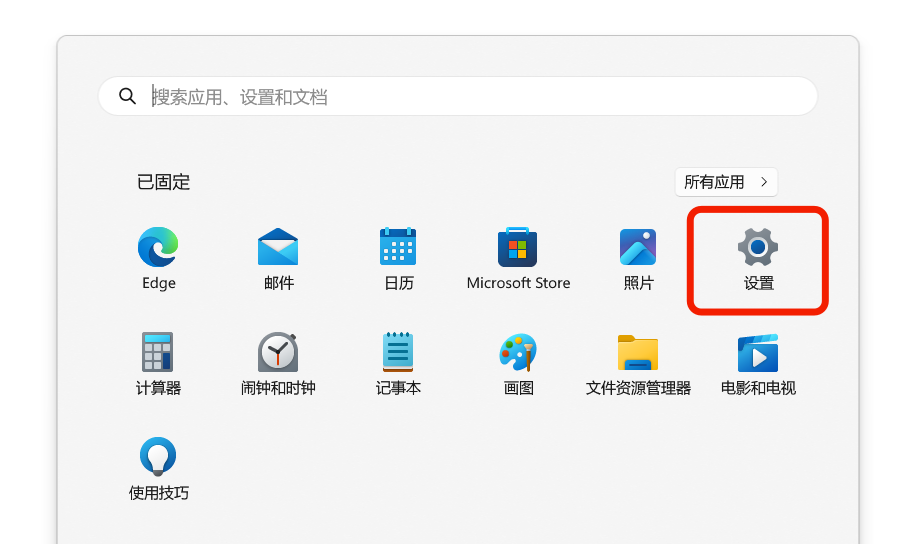
\includegraphics[width=.6\textwidth]{assets/basic/Settings.png}
  \caption{设置}
  \label{fig:Settings}
\end{figure}

你可能听说过「控制面板」这个词,它是 Windows 10 之前的 Windows 系统中用来调整系统设置的应用。在今天我们常用的 Windows 10 和 Windows 11 中,控制面板仍然存在,但它的功能已经被「设置」app 取代。只有当我们在文中明确使用「控制面板」一词时,才需要你使用它。

\practice

\begin{enumerate}
  \item 计算 1 GB 等于多少 KB?等于多少字节?假设一个汉字占两个字节,1 GB 大约可以记录多少个汉字?
  \item 尝试计算,一个按 1000 进位计算得到容量为 64 GB 的 U 盘,按 1024 进位计算得到的容量是多少?
  \item 在自己电脑上尝试这些快捷键:
    \begin{enumerate}
      \item \keys{\Windows + Shift + S} (仅限 Windows 10 / 11)
      \item \keys{Ctrl + Shift + Esc}
      \item \keys{\Windows + D}
    \end{enumerate}
  \item 如果你在用笔记本电脑,了解并体验它 \keys{F1} -- \keys{F12} 功能键的扩展功能。
\end{enumerate}